\begin{figure*}
        \centering
        \begin{subfigure}[b]{0.475\textwidth}
            \centering
            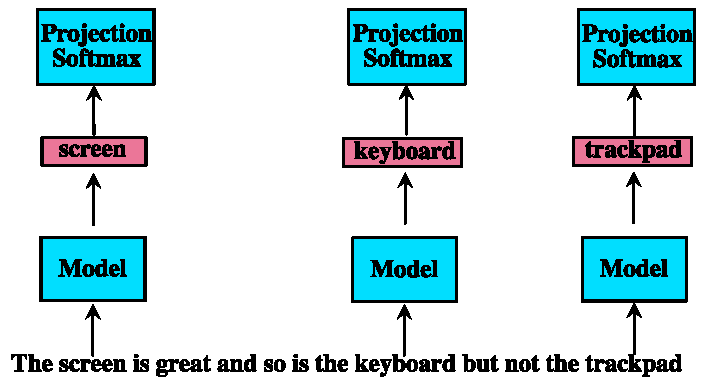
\includegraphics[width=\textwidth]{images/augmentation/methods_performance/Inter_Target/normal.pdf}
            \caption{General non-target aware setup.}    
            \label{fig:aug_normal_target_modelling}
        \end{subfigure}
        \hfill
        \begin{subfigure}[b]{0.475\textwidth}  
            \centering 
            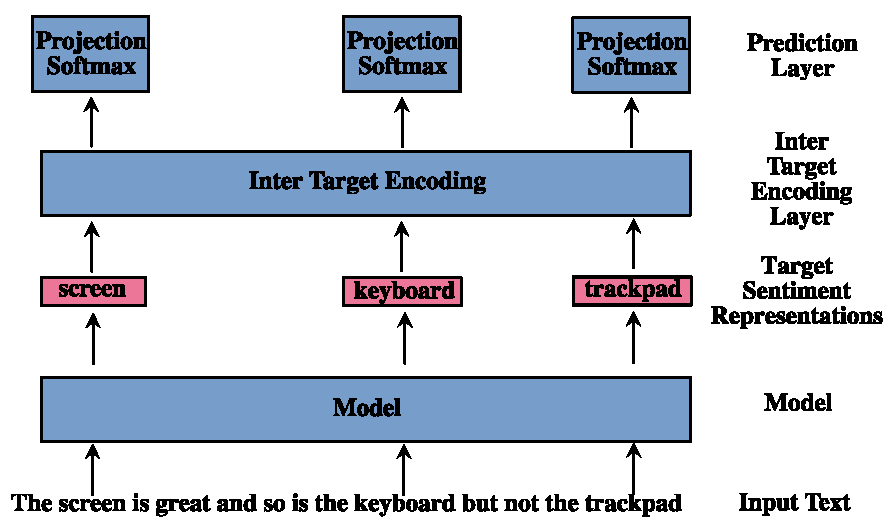
\includegraphics[width=\textwidth]{images/augmentation/methods_performance/Inter_Target/inter_target_encoding.pdf}
            \caption{General target aware setup.}    
            \label{fig:aug_target_general_modelling}
        \end{subfigure}
        \vskip\baselineskip
        \begin{subfigure}[b]{0.475\textwidth}   
            \centering 
            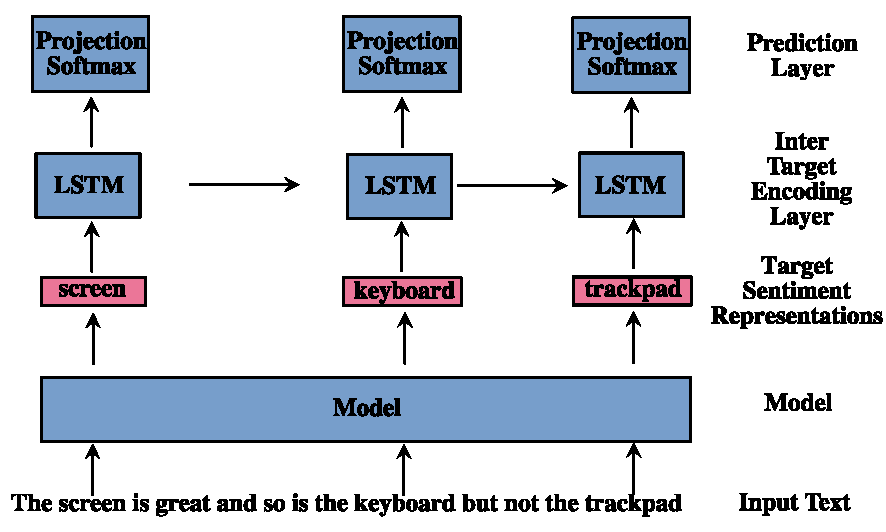
\includegraphics[width=\textwidth]{images/augmentation/methods_performance/Inter_Target/LSTM_Encdoing.pdf}
            \caption{Target aware setup of \citet{hazarika-etal-2018-modeling}.}    
            \label{fig:aug_target_hazarika_modelling}
        \end{subfigure}
        \quad
        \begin{subfigure}[b]{0.475\textwidth}   
            \centering 
            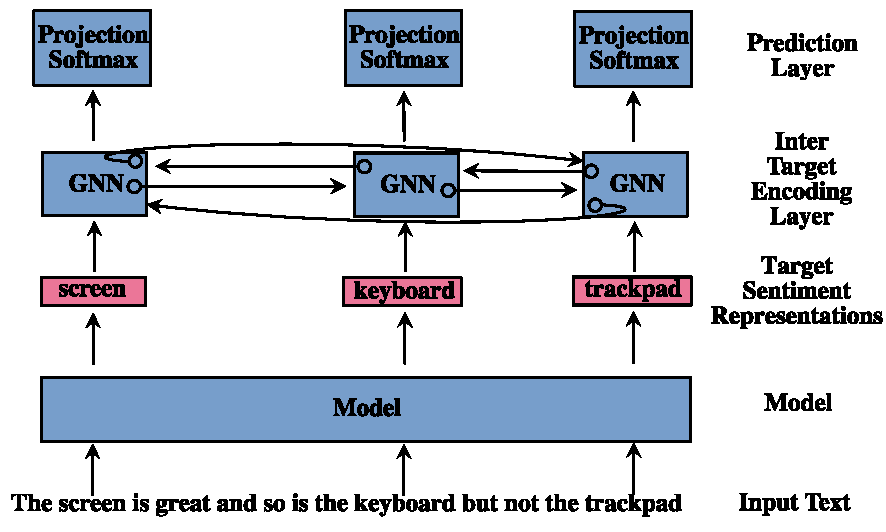
\includegraphics[width=\textwidth]{images/augmentation/methods_performance/Inter_Target/GNN_Encoding.pdf}
            \caption{Target aware setup of \citet{zhao2019modeling}.}    
            \label{fig:aug_target_zhao_modelling}
        \end{subfigure}
        \caption{The first row shows in abstract the difference between non target aware and aware setups. The second row shows more concrete target aware methods.} 
        \label{fig:aug_target_aware_and_non_setups}
\end{figure*}